\documentclass[12pt, a4paper]{article}
\usepackage[utf8]{inputenc}
\usepackage{geometry}
\usepackage{titlesec}
\usepackage{tocloft}
\usepackage{enumitem}
\usepackage{hyperref}
\usepackage{graphicx}
\usepackage{fancyhdr}
\usepackage{amsmath}
\usepackage{amssymb}
\usepackage{float}
\usepackage{array}
\usepackage{booktabs}
\usepackage{longtable}
\usepackage[most]{tcolorbox}
\usepackage{listings}
\usepackage{xcolor}

% Page Geometry
\geometry{
    a4paper,
    total={170mm,257mm},
    left=20mm,
    top=25mm,
}

\setlength{\headheight}{15pt}

% Hyperlink Setup
\hypersetup{
    colorlinks=true,
    linkcolor=black,
    filecolor=magenta,
    urlcolor=blue,
    citecolor=blue
}

% Header and Footer
\pagestyle{fancy}
\fancyhf{}
\rhead{Airline Reservation System - Phase 2}
\lhead{DBMS Project Report}
\cfoot{\thepage}

\renewcommand{\cftsecdotsep}{\cftdotsep}
\tocloftpagestyle{fancy}

%SQL-Listing Style
\lstdefinestyle{sqlstyle}{
    language=SQL,
    basicstyle=\ttfamily\small,
    keywordstyle=\color{blue},
    commentstyle=\color{gray},
    stringstyle=\color{teal},
    showstringspaces=false,
    breaklines=true,
    frame=single
}

\begin{document}

\begin{titlepage}
    \centering

    \IfFileExists{logo.png}{
        \begin{tabular}{c}
            
\includegraphics[width=0.25\textwidth]{logo.png} \\
            \vspace{0.1cm}
        \end{tabular}
    }{
        \framebox{\parbox{0.3\textwidth}{\centering \vspace{1cm} Logo Here \vspace{1cm}}}
    }

    \vspace{1.5cm}

    \hrule height 1pt
    \vspace{0.4cm}
    {\Large \textbf{\MakeUppercase{A DBMS Project On}}} \\
    \vspace{0.4cm}
    \hrule height 1pt

    \vspace{1cm}

    \begin{tcolorbox}[
        colback=black,
        coltext=white,
        colframe=black,
        arc=0mm,
        boxrule=0pt,
        halign=center,
        width=1\textwidth,
        top=10mm, bottom=10mm
    ]
        \fontsize{20}{24}\selectfont \textbf{\MakeUppercase{Design and Implementation of an}} \\[0.5cm]
        \fontsize{20}{24}\selectfont \textbf{\MakeUppercase{Airline Reservation System}} \\[0.4cm]
        \fontsize{16}{20}\selectfont \textbf{\MakeUppercase{Phase II Report}}
    \end{tcolorbox}

    \vspace{1cm}

    {\Large \textbf{\MakeUppercase{Submitted By}}}

    \vspace{0.5cm}

    \begin{tcolorbox}[
        colback=white,
        colframe=black,
        boxrule=1pt,
        arc=0mm,
        width=0.9\textwidth
    ]
        \centering
        \renewcommand{\arraystretch}{1.5}
        \begin{tabular}{r l}
            \textbf{Names:} & \textbf{Paranjoy Bordoloi  (24070122129)} \\
                            & \textbf{Parmar Divyaansh  (24070122130)} \\
                            & \textbf{Parth Sarathi Giri  (24070122132)} \\
            \textbf{Batch:} & 2024 - 2028 \\
            \textbf{Faculty:} & Prof. Jitendra Rajpurohit
        \end{tabular}
    \end{tcolorbox}

    \vspace{2cm}
    {\text{{Department of Computer Science}}}\\
    {\text{{Symbiosis Institute of Technology, Pune}}}
\end{titlepage}

\tableofcontents
\newpage



\section{Introduction}

\subsection{Contextual Overview of Airline Data Management}
The airline domain is a high-volume transactional environment where booking requests, schedule updates, seat inventory changes, and payment confirmations occur continuously. In such a setting, a weak data model quickly leads to duplicate records, inconsistent seat availability, and delayed operational visibility for both passengers and administrators. The Airline Reservation System in this project is designed around a normalized relational core so that operational data remains consistent under concurrent access and frequent updates.

From a DBMS perspective, airline operations are not only about storing bookings; they require strict entity separation (passenger, flight, route, aircraft, payment), reliable foreign-key relationships, and procedural controls for event-driven validation. This report follows that direction and demonstrates how schema design and database logic are applied to meet practical reservation workflows.

\subsection{Evolution from Phase I Design to Phase II Implementation}
Phase I established the conceptual and logical foundation through ER/EER modeling, relationship analysis, and normalization planning. Phase II advances this foundation into executable implementation by delivering full schema scripts, trigger/procedure logic, test data flows, and query-result demonstrations.

The final implementation uses a shared MySQL schema accessed by two application layers:
\begin{itemize}
    \item Passenger and booking APIs through FastAPI.
    \item Admin and analytics operations through a Java/Tomcat module and Java CLI.
\end{itemize}
Both modules use the same normalized database, ensuring that validation, consistency, and reporting depend on one authoritative relational state.

\subsection{Project Scope and Objectives in Phase II}
Phase II focuses on end-to-end verifiable database execution, not only theory. The scope includes:
\begin{itemize}
    \item Implementing the complete relational schema in MySQL.
    \item Enforcing integrity using constraints, triggers, and procedures.
    \item Demonstrating anomaly prevention through normalized decomposition.
    \item Verifying behavior with query-output evidence from the implemented state.
\end{itemize}

Primary implementation assets used in this report are:
\begin{itemize}
    \item \texttt{database/01\_schema.sql}
    \item \texttt{database/02\_triggers.sql}
    \item \texttt{database/03\_seed.sql}
\end{itemize}

\section{About the Project}
The Airline Reservation System is implemented as a dual-backend full-stack project with a normalized MySQL database at its core. Passenger transactions are handled by FastAPI services, admin summary APIs are exposed through a Java/Tomcat module, and both are backed by the same relational schema.

\section{Addressed Pain Points}
\begin{itemize}
    \item Preventing seat double-booking in concurrent booking attempts.
    \item Preventing overlapping aircraft schedules.
    \item Maintaining accurate seat inventory after booking/cancellation transitions.
    \item Separating identity, transaction, and operational logs to avoid redundancy and update drift.
    \item Enabling admin-level filtered booking analysis by status, flight, and passenger dimensions.
\end{itemize}

\section{EER Diagram}
\begin{figure}[H]
    \centering
    \IfFileExists{new.png}{
        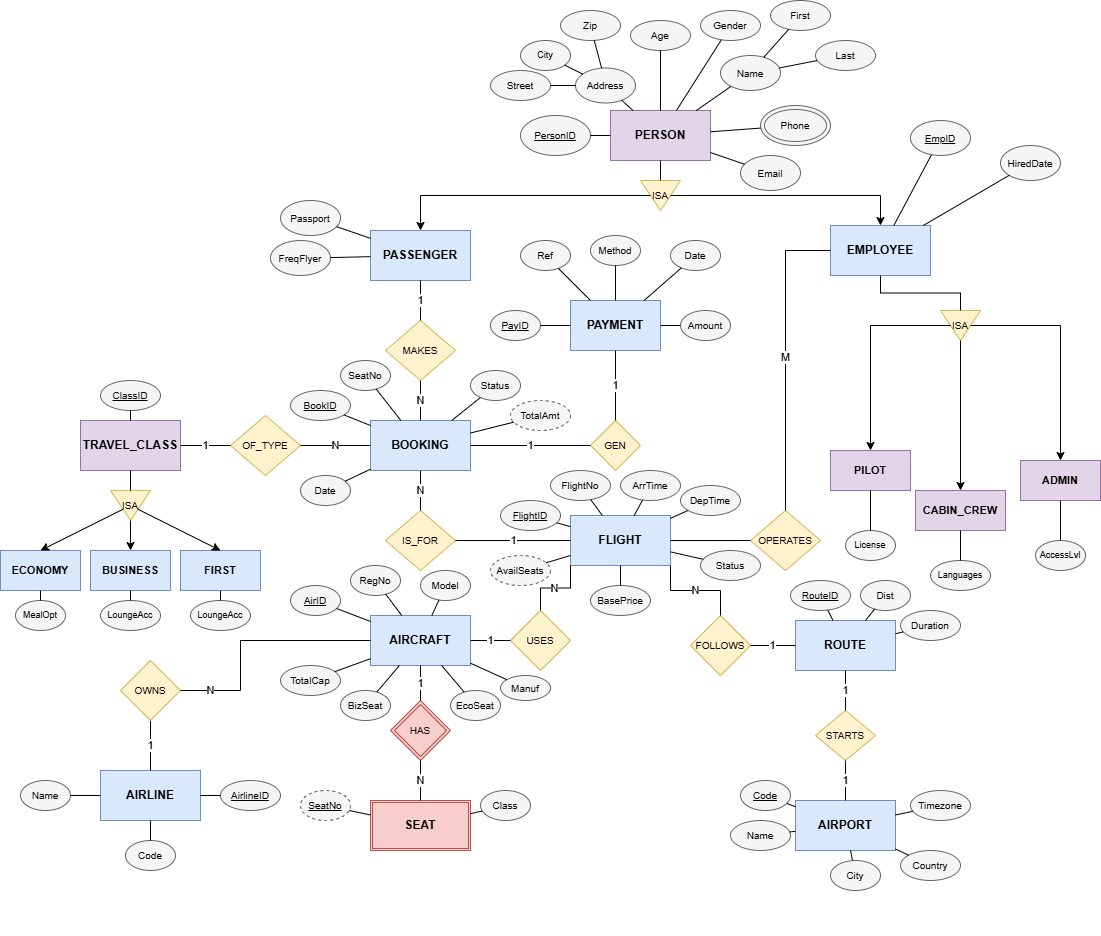
\includegraphics[width=0.95\textwidth]{eer_diagram2}
    }{
        \framebox{\parbox{0.85\textwidth}{\centering
            \vspace{2.5cm}
            \textbf{ER diagram placeholder (eer_diagram2.png not found).} \\
            Add the final ER/EER image as \texttt{eer_diagram2.png} in project root.
            \vspace{2.5cm}
        }}
    }
    \caption{EER representation of the implemented airline reservation schema.}
\end{figure}

\newpage
\section{Anomalies Identified in Flat (Denormalized) Design}

The following anomalies are present in a flat, denormalized booking structure where all passenger, flight, airport, and seat information is stored together in a single relation:

\begin{lstlisting}[style=sqlstyle,caption={Denormalized design (used for anomaly identification only)}]
CREATE TABLE booking_flat_before (
    booking_reference VARCHAR(12) PRIMARY KEY,
    passenger_name VARCHAR(100),
    passenger_email VARCHAR(100),
    passport_number VARCHAR(20),
    flight_number VARCHAR(10),
    origin_code VARCHAR(3),
    dest_code VARCHAR(3),
    departure_time DATETIME,
    arrival_time DATETIME,
    aircraft_registration VARCHAR(20),
    aircraft_model VARCHAR(50),
    total_capacity INT,
    seat_number VARCHAR(5),
    class_type VARCHAR(20),
    total_amount DECIMAL(10,2),
    booking_status VARCHAR(20)
);
\end{lstlisting}

\textbf{Anomalies present:}
\begin{itemize}
    \item \textbf{Insertion anomaly}: A new passenger cannot be recorded unless they have also booked a flight (forced dummy rows).
    \item \textbf{Update anomaly}: Changing a single airport name or aircraft model requires updating many booking rows, risking inconsistency.
    \item \textbf{Deletion anomaly}: Cancelling the only booking for a route erases route/flight/aircraft history from the relation.
    \item \textbf{Seat conflict anomaly}: No mechanism to prevent duplicate seat assignment for the same flight by concurrent transactions.
    \item \textbf{Capacity overrun}: No automated guard against overbooking beyond aircraft capacity.
\end{itemize}

\section{Functional Dependencies}

\subsection{Core Dependencies}
\footnotesize
\begin{longtable}{|p{0.41\textwidth}|p{0.51\textwidth}|}
\hline
\textbf{Functional Dependency Rule} & \textbf{Interpretation} \\
\hline
\texttt{airline\_id} $\rightarrow$ \texttt{name, code} & Airline identifier determines airline name and airline code. \\
\hline
\texttt{code} $\rightarrow$ \texttt{airline\_id, name} & Airline code is also a candidate key for airline data. \\
\hline
\texttt{airport\_code} $\rightarrow$ \texttt{name, city, country, timezone} & Airport code determines all airport attributes. \\
\hline
\texttt{route\_id} $\rightarrow$ \texttt{origin\_code, dest\_code, distance\_km, estimated\_duration\_minutes} & Route identifier determines origin-destination path details. \\
\hline
\texttt{aircraft\_id} $\rightarrow$ \texttt{registration\_number, model, manufacturer, total\_capacity, business\_seats, economy\_seats, airline\_id} & Aircraft identifier determines full aircraft profile. \\
\hline
\texttt{registration\_number} $\rightarrow$ \texttt{aircraft\_id, model, manufacturer, total\_capacity, business\_seats, economy\_seats, airline\_id} & Registration number uniquely determines the aircraft record. \\
\hline
\texttt{flight\_id} $\rightarrow$ \texttt{flight\_number, route\_id, aircraft\_id, departure\_time, arrival\_time, base\_price, status, available\_seats} & Flight identifier determines all flight-level facts. \\
\hline
\texttt{passenger\_id} $\rightarrow$ \texttt{first\_name, last\_name, email, phone, passport\_number, date\_of\_birth, address, frequent\_flyer\_number} & Passenger identifier determines complete passenger profile. \\
\hline
\texttt{email (passenger)} $\rightarrow$ \texttt{passenger\_id, first\_name, last\_name, phone, passport\_number, date\_of\_birth, address, frequent\_flyer\_number} & Email acts as a candidate key for passenger lookup. \\
\hline
\texttt{passport\_number} $\rightarrow$ \texttt{passenger\_id, first\_name, last\_name, email, phone, date\_of\_birth, address, frequent\_flyer\_number} & Passport number acts as another candidate key for passenger. \\
\hline
\texttt{user\_id} $\rightarrow$ \texttt{passenger\_id, employee\_id, email, password\_hash, role, is\_active, created\_at} & Application user identifier determines authentication and role fields. \\
\hline
\texttt{booking\_id} $\rightarrow$ \texttt{booking\_reference, passenger\_id, flight\_id, booking\_date, seat\_number, class\_type, status, total\_amount, cancellation\_time} & Booking identifier determines booking lifecycle attributes. \\
\hline
\texttt{booking\_reference} $\rightarrow$ \texttt{booking\_id, passenger\_id, flight\_id, booking\_date, seat\_number, class\_type, status, total\_amount, cancellation\_time} & Booking reference is a candidate key for booking records. \\
\hline
\texttt{(flight\_id, seat\_number)} $\rightarrow$ \texttt{booking\_id} & Composite key ensures a seat maps to at most one booking per flight. \\
\hline
\texttt{payment\_id} $\rightarrow$ \texttt{booking\_id, amount, payment\_method, transaction\_date, transaction\_reference, payment\_status} & Payment identifier determines payment transaction details. \\
\hline
\texttt{booking\_id (payment)} $\rightarrow$ \texttt{payment\_id, amount, payment\_method, transaction\_date, transaction\_reference, payment\_status} & Booking identifier can determine its associated payment row. \\
\hline
\texttt{transaction\_reference} $\rightarrow$ \texttt{payment\_id, booking\_id, amount, payment\_method, transaction\_date, payment\_status} & Transaction reference uniquely identifies a payment transaction. \\
\hline
\texttt{refund\_id} $\rightarrow$ \texttt{booking\_id, refund\_amount, reason, processed\_at, refund\_status} & Refund identifier determines refund processing details. \\
\hline
\end{longtable}
\normalsize

\section{Normalization Applied to Updated Tables}

\subsection{UNF to 1NF: Atomic Attributes and Functional Dependency Clarification}

\textbf{Objective:} Eliminate repeating groups and ensure all attributes are atomic (single-valued, indivisible).

\textbf{Before (UNF):} Booking table contains non-atomic and multi-valued elements:
\begin{center}
\small
\begin{tabular}{|c|c|c|c|}
\hline
\textbf{booking\_ref} & \textbf{passenger\_info} & \textbf{flight\_info} & \textbf{seat\_details} \\
\hline
PNR00000001 & Paranjoy Bordoloi, 9999000001, P1234567 & AI201, DEL, BOM & 12A, Economy \\
\hline
\end{tabular}
\end{center}

\textbf{After (1NF):} Each attribute is atomic and belongs to exactly one table:

\begin{lstlisting}[style=sqlstyle]
-- Passenger table
CREATE TABLE passenger (
    passenger_id INT AUTO_INCREMENT PRIMARY KEY,
    first_name VARCHAR(50) NOT NULL,
    last_name VARCHAR(50) NOT NULL,
    email VARCHAR(100) UNIQUE NOT NULL,
    phone VARCHAR(15),
    passport_number VARCHAR(20) UNIQUE NOT NULL,
    date_of_birth DATE,
    address VARCHAR(255),
    frequent_flyer_number VARCHAR(30) UNIQUE
);

-- Flight table (atomic: one row per flight)
CREATE TABLE flight (
    flight_id INT AUTO_INCREMENT PRIMARY KEY,
    flight_number VARCHAR(10) NOT NULL,
    route_id INT NOT NULL,
    aircraft_id INT NOT NULL,
    departure_time DATETIME NOT NULL,
    arrival_time DATETIME NOT NULL,
    base_price DECIMAL(10, 2) NOT NULL,
    status ENUM('Scheduled', 'Boarding', 'Departed', 'Cancelled') DEFAULT 'Scheduled',
    available_seats INT NOT NULL,
    FOREIGN KEY (route_id) REFERENCES route(route_id),
    FOREIGN KEY (aircraft_id) REFERENCES aircraft(aircraft_id)
);

-- Booking table (atomic: one booking per row)
CREATE TABLE booking (
    booking_id INT AUTO_INCREMENT PRIMARY KEY,
    booking_reference VARCHAR(12) UNIQUE NOT NULL,
    passenger_id INT NOT NULL,
    flight_id INT NOT NULL,
    booking_date DATETIME DEFAULT CURRENT_TIMESTAMP,
    seat_number VARCHAR(5),
    class_type ENUM('Economy', 'Business', 'First') NOT NULL,
    status ENUM('Pending', 'Confirmed', 'Cancelled') NOT NULL,
    total_amount DECIMAL(10, 2) NOT NULL,
    cancellation_time DATETIME,
    FOREIGN KEY (passenger_id) REFERENCES passenger(passenger_id),
    FOREIGN KEY (flight_id) REFERENCES flight(flight_id),
    UNIQUE KEY uq_flight_seat (flight_id, seat_number)
);
\end{lstlisting}

\textbf{Benefit:} All values are now single-valued and non-repeating, enabling proper relational operations.

\subsection{1NF to 2NF: Eliminate Partial Dependencies}

\textbf{Objective:} Remove partial dependencies where non-key attributes depend on part of a composite key instead of the entire key.

\textbf{Before (1NF with partial dependencies):} If aircraft details were stored together with flight:
\begin{center}
\small
\begin{tabular}{|c|c|c|c|c|c|}
\hline
\textbf{flight\_id} & \textbf{aircraft\_id} & \textbf{aircraft\_model} & \textbf{manufacturer} & \textbf{capacity} & \textbf{departure\_time} \\
\hline
1 & 1 & Boeing 737 & Boeing & 180 & 2026-03-15 08:00 \\
\hline
2 & 1 & Boeing 737 & Boeing & 180 & 2026-03-15 14:00 \\
\hline
\end{tabular}
\end{center}

Aircraft repetition: same aircraft duplicated across multiple flights. Changing manufacturer requires multiple updates.

\textbf{After (2NF):} Aircraft attributes moved to a separate \texttt{aircraft} table, referenced by foreign key:

\begin{lstlisting}[style=sqlstyle]
-- Aircraft master table (no partial dependencies)
CREATE TABLE aircraft (
    aircraft_id INT AUTO_INCREMENT PRIMARY KEY,
    registration_number VARCHAR(20) UNIQUE NOT NULL,
    model VARCHAR(50) NOT NULL,
    manufacturer VARCHAR(50) NOT NULL,
    total_capacity INT NOT NULL,
    business_seats INT,
    economy_seats INT,
    airline_id INT NOT NULL,
    FOREIGN KEY (airline_id) REFERENCES airline(airline_id)
);

-- Flight table now only contains aircraft_id foreign key
CREATE TABLE flight (
    flight_id INT AUTO_INCREMENT PRIMARY KEY,
    flight_number VARCHAR(10) NOT NULL,
    route_id INT NOT NULL,
    aircraft_id INT NOT NULL,  -- References aircraft table
    departure_time DATETIME NOT NULL,
    arrival_time DATETIME NOT NULL,
    base_price DECIMAL(10, 2) NOT NULL,
    status ENUM('Scheduled', 'Boarding', 'Departed', 'Cancelled') DEFAULT 'Scheduled',
    available_seats INT NOT NULL,
    FOREIGN KEY (route_id) REFERENCES route(route_id),
    FOREIGN KEY (aircraft_id) REFERENCES aircraft(aircraft_id)
);
\end{lstlisting}

\textbf{Example:} Update aircraft model in one location only:
\begin{lstlisting}[style=sqlstyle]
-- Before: Update needed in every booking row and flight row
UPDATE flight SET aircraft_model = 'Boeing 737 MAX 9' WHERE aircraft_id = 1;

-- After (2NF): Single update in aircraft table
UPDATE aircraft SET model = 'Boeing 737 MAX 9' WHERE aircraft_id = 1;
\end{lstlisting}

\textbf{Benefit:} Non-key attributes now depend on the entire primary key, not part of it. This solves the \textbf{update anomaly}.

\subsection{2NF to 3NF: Eliminate Transitive Dependencies}

\textbf{Objective:} Remove transitive dependencies where non-key attributes depend on other non-key attributes rather than directly on the primary key.

\textbf{Before (2NF with transitive dependencies):} If route details were stored in the flight table:
\begin{center}
\small
\begin{tabular}{|c|c|c|c|c|}
\hline
\textbf{flight\_id} & \textbf{route\_id} & \textbf{origin\_code} & \textbf{dest\_code} & \textbf{distance\_km} \\
\hline
1 & 1 & DEL & BOM & 1474 \\
\hline
2 & 1 & DEL & BOM & 1474 \\
\hline
3 & 1 & DEL & BOM & 1474 \\
\hline
\end{tabular}
\end{center}

Transitive: \({\rm flight\_id} \rightarrow {\rm route\_id} \rightarrow \{{\rm origin\_code}, {\rm dest\_code}, {\rm distance\_km}\}\).

Deleting the last flight on DEL--BOM route loses route information entirely.

\textbf{After (3NF):} Route and airport attributes isolated in separate tables:

\begin{lstlisting}[style=sqlstyle]
-- Airport master table
CREATE TABLE airport (
    airport_code VARCHAR(3) PRIMARY KEY,
    name VARCHAR(100) NOT NULL,
    city VARCHAR(50) NOT NULL,
    country VARCHAR(50) NOT NULL,
    timezone VARCHAR(10)
);

-- Route master table
CREATE TABLE route (
    route_id INT AUTO_INCREMENT PRIMARY KEY,
    origin_code VARCHAR(3) NOT NULL,
    dest_code VARCHAR(3) NOT NULL,
    distance_km DECIMAL(6, 2),
    estimated_duration_minutes INT,
    FOREIGN KEY (origin_code) REFERENCES airport(airport_code),
    FOREIGN KEY (dest_code) REFERENCES airport(airport_code),
    UNIQUE KEY uq_route (origin_code, dest_code)
);

-- Flight table no longer contains transitive attributes
CREATE TABLE flight (
    flight_id INT AUTO_INCREMENT PRIMARY KEY,
    flight_number VARCHAR(10) NOT NULL,
    route_id INT NOT NULL,
    aircraft_id INT NOT NULL,
    departure_time DATETIME NOT NULL,
    arrival_time DATETIME NOT NULL,
    base_price DECIMAL(10, 2) NOT NULL,
    status ENUM('Scheduled', 'Boarding', 'Departed', 'Cancelled') DEFAULT 'Scheduled',
    available_seats INT NOT NULL,
    FOREIGN KEY (route_id) REFERENCES route(route_id),
    FOREIGN KEY (aircraft_id) REFERENCES aircraft(aircraft_id)
);
\end{lstlisting}

\textbf{Example:} Update airport information without affecting flights:
\begin{lstlisting}[style=sqlstyle]
-- Before (2NF): Modify origin/dest details in every flight row (error-prone)
UPDATE flight SET destination_city = 'Mumbai' WHERE dest_code = 'BOM';  -- Inconsistency risk

-- After (3NF): Single update in airport table
UPDATE airport SET city = 'Mumbai' WHERE airport_code = 'BOM';
\end{lstlisting}

\textbf{Benefit:} All non-key attributes depend directly on the primary key, not transitively on other non-key attributes. This solves the \textbf{update and deletion anomalies}.

\subsection{3NF Refinement: Business Logic and Concurrency}

The following additional tables complete the 3NF design:

\begin{lstlisting}[style=sqlstyle]
-- Payment lifecycle (separates transactional state from booking state)
CREATE TABLE payment (
    payment_id INT AUTO_INCREMENT PRIMARY KEY,
    booking_id INT NOT NULL,
    amount DECIMAL(10, 2) NOT NULL,
    payment_method ENUM('Credit Card', 'Debit Card', 'UPI', 'Net Banking') NOT NULL,
    transaction_date DATETIME DEFAULT CURRENT_TIMESTAMP,
    transaction_reference VARCHAR(50),
    payment_status ENUM('Pending', 'Completed', 'Failed', 'Refunded') NOT NULL,
    FOREIGN KEY (booking_id) REFERENCES booking(booking_id)
);

-- Refund lifecycle (separates refund state from booking cancellation)
CREATE TABLE refund (
    refund_id INT AUTO_INCREMENT PRIMARY KEY,
    booking_id INT NOT NULL,
    refund_amount DECIMAL(10, 2) NOT NULL,
    reason VARCHAR(255),
    processed_at DATETIME DEFAULT CURRENT_TIMESTAMP,
    refund_status ENUM('Pending', 'Completed', 'Rejected') NOT NULL,
    FOREIGN KEY (booking_id) REFERENCES booking(booking_id)
);

-- Seat locks for concurrency control (solves seat conflict anomaly)
CREATE TABLE seat_lock (
    lock_id INT AUTO_INCREMENT PRIMARY KEY,
    flight_id INT NOT NULL,
    seat_number VARCHAR(5) NOT NULL,
    passenger_id INT NOT NULL,
    locked_at DATETIME DEFAULT CURRENT_TIMESTAMP,
    expires_at DATETIME NOT NULL,
    FOREIGN KEY (flight_id) REFERENCES flight(flight_id),
    FOREIGN KEY (passenger_id) REFERENCES passenger(passenger_id),
    UNIQUE KEY uq_flight_seat_lock (flight_id, seat_number)
);
\end{lstlisting}

\subsection{Normalization Impact on Anomalies}
\begin{center}
\begin{longtable}{|p{0.22\textwidth} |p{0.33\textwidth} |p{0.38\textwidth}|}
	\hline
	\textbf{Anomaly} & \textbf{Root Cause (Denormalized)} & \textbf{Solution (Normalized 3NF)} \\
	\hline
	\textbf{Insertion} & Passenger/flight/route cannot be inserted independently; forced dummy rows required. & Separate \texttt{passenger}, \texttt{route}, \texttt{aircraft}, \texttt{airport} tables allow independent insertions. \\
	\hline
	\textbf{Update} & Changing airport name or aircraft model requires updating multiple booking/flight rows. & Single master-table update propagates through FK relationships. \\
	\hline
	\textbf{Deletion} & Deleting the only booking for a route erases route/flight history. & Deleting a booking does not cascade to \texttt{route}, \texttt{flight}, or \texttt{aircraft} tables. \\
	\hline
	\textbf{Seat Conflict} & Multiple bookings for same (flight, seat) can occur without constraint checking. & \texttt{UNIQUE KEY (flight\_id, seat\_number)} and \texttt{seat\_lock} trigger prevent duplicates. \\
	\hline
	\textbf{Capacity Overrun} & No guard against exceeding aircraft capacity. & Trigger \texttt{tr\_booking\_before\_insert} checks available\_seats and rejects overbooking. \\
	\hline
	\textbf{Schedule Overlap} & Same aircraft assigned to overlapping time blocks. & Trigger \texttt{tr\_flight\_before\_insert} validates aircraft is not in use during departure/arrival window. \\
	\hline
\end{longtable}

\end{center}
\newpage
\section{Implementation of Tables in MySQL/Oracle}

\subsection{MySQL Implementation}
The complete table implementation used in project execution is included below.

\lstinputlisting[style=sqlstyle,caption={Complete table creation script (MySQL)}]{database/01_schema.sql}

\subsection{Oracle Adaptation Notes}
\begin{itemize}
    \item Use \texttt{GENERATED AS IDENTITY} or sequences in place of \texttt{AUTO\_INCREMENT}.
    \item Replace MySQL \texttt{ENUM} with \texttt{VARCHAR2} + \texttt{CHECK} constraints.
    \item Keep table decomposition, keys, and dependency design unchanged.
\end{itemize}

\section{Execution of Queries, Functions/Procedures, and Triggers}

\subsection{Complete Trigger and Procedure Code Used}
\lstinputlisting[style=sqlstyle,caption={Complete trigger + procedure implementation}]{database/02_triggers.sql}

\subsection{Test Data Insertion}

Before executing queries and demonstrating triggers/procedures, the following data is inserted:

\textbf{Step 1: Insert Master Data (Airport)}
\begin{lstlisting}[style=sqlstyle]
INSERT INTO airport (airport_code, name, city, country, timezone) VALUES
('DEL', 'Indira Gandhi International Airport', 'New Delhi', 'India', 'IST'),
('BOM', 'Bombay High Airport', 'Mumbai', 'India', 'IST'),
('BLR', 'Kempegowda International Airport', 'Bangalore', 'India', 'IST'),
('PNQ', 'Pune Airport', 'Pune', 'India', 'IST'),
('GOI', 'Dabolim Airport', 'Goa', 'India', 'IST'),
('LHR', 'London Heathrow', 'London', 'UK', 'GMT'),
('CDG', 'Paris Charles de Gaulle', 'Paris', 'France', 'CEST');
\end{lstlisting}

\textbf{Step 2: Insert Routes}
\begin{lstlisting}[style=sqlstyle]
INSERT INTO route (origin_code, dest_code, distance_km, estimated_duration_minutes) VALUES
('DEL', 'BOM', 1474, 150),
('DEL', 'BLR', 2150, 180),
('BOM', 'PNQ', 180, 45),
('BLR', 'GOI', 450, 75),
('DEL', 'LHR', 7210, 540),
('CDG', 'DEL', 8350, 570);
\end{lstlisting}

\textbf{Step 3: Insert Airlines}
\begin{lstlisting}[style=sqlstyle]
INSERT INTO airline (name, code, country) VALUES
('Air India', 'AI', 'India'),
('IndiGo', '6E', 'India'),
('Vistara', 'UK', 'India'),
('British Airways', 'BA', 'UK'),
('Air France', 'AF', 'France');
\end{lstlisting}

\textbf{Step 4: Insert Aircraft}
\begin{lstlisting}[style=sqlstyle]
INSERT INTO aircraft (registration_number, model, manufacturer, total_capacity, 
                       business_seats, economy_seats, airline_id) VALUES
('VT-AEP', 'Boeing 777-300ER', 'Boeing', 374, 30, 344, 1),
('VT-IGC', 'Airbus A320', 'Airbus', 180, 12, 168, 2),
('N904BA', 'Boeing 787-9', 'Boeing', 296, 42, 254, 4),
('F-GZCO', 'Airbus A380', 'Airbus', 555, 76, 479, 5);
\end{lstlisting}

\textbf{Step 5: Insert Flights}
\begin{lstlisting}[style=sqlstyle]
INSERT INTO flight (flight_number, route_id, aircraft_id, departure_time, 
                     arrival_time, base_price, status, available_seats) VALUES
('AI201', 1, 1, '2026-03-15 08:00:00', '2026-03-15 10:30:00', 6200.00, 'Scheduled', 374),
('6E402', 1, 2, '2026-03-15 12:00:00', '2026-03-15 14:30:00', 4800.00, 'Scheduled', 180),
('AI203', 2, 1, '2026-03-15 15:00:00', '2026-03-15 18:00:00', 7500.00, 'Scheduled', 374),
('UK405', 3, 2, '2026-03-16 09:00:00', '2026-03-16 10:00:00', 2500.00, 'Scheduled', 180),
('BA101', 5, 3, '2026-03-20 22:00:00', '2026-03-21 10:00:00', 55000.00, 'Scheduled', 296),
('AF501', 6, 4, '2026-03-25 18:00:00', '2026-03-26 06:00:00', 85000.00, 'Scheduled', 555);
\end{lstlisting}

\textbf{Step 6: Insert Passengers}
\begin{lstlisting}[style=sqlstyle]
INSERT INTO passenger (first_name, last_name, email, phone, passport_number, 
                        date_of_birth, address, frequent_flyer_number) VALUES
('Paranjoy', 'Bordoloi', 'paranjoy@example.com', '9999000001', 'P1234567', 
 '1999-05-15', 'Delhi, India', 'PARAN001'),
('Divyaansh', 'Parmar', 'divyaansh@example.com', '9999000002', 'P2234562', 
 '2000-08-22', 'Mumbai, India', 'DIVYA002'),
('Parth', 'Giri', 'parth@example.com', '9999000003', 'P3234563', 
 '1998-12-10', 'Bangalore, India', 'PARTH003'),
('Ira', 'Menon', 'ira.menon@example.com', '9999000055', 'P4234564', 
 '1994-01-27', 'Delhi, India', 'IRA004'),
('Rajesh', 'Kumar', 'rajesh@example.com', '9999000005', 'P5234565', 
 '1995-06-14', 'Pune, India', 'RAJESH05');
\end{lstlisting}

\textbf{Step 7: Insert App Users (with hashed passwords)}
\begin{lstlisting}[style=sqlstyle]
INSERT INTO app_user (passenger_id, email, password_hash, role, is_active) VALUES
(1, 'paranjoy@example.com', '$2b$12$hashedpwd1', 'passenger', 1),
(2, 'divyaansh@example.com', '$2b$12$hashedpwd2', 'passenger', 1),
(3, 'parth@example.com', '$2b$12$hashedpwd3', 'passenger', 1),
(4, 'ira.menon@example.com', '$2b$12$hashedpwd4', 'passenger', 1),
(5, 'rajesh@example.com', '$2b$12$hashedpwd5', 'passenger', 1);
\end{lstlisting}

\subsection{Sample Database State After Insertions}

\textbf{Airport Table (7 rows)}
\begin{center}
\small
\begin{tabular}{|c|c|c|c|c|}
\hline
\textbf{airport\_code} & \textbf{name} & \textbf{city} & \textbf{country} & \textbf{timezone} \\
\hline
DEL & Indira Gandhi International... & New Delhi & India & IST \\
\hline
BOM & Bombay High Airport & Mumbai & India & IST \\
\hline
BLR & Kempegowda International... & Bangalore & India & IST \\
\hline
\multicolumn{5}{|c|}{... (4 more rows: PNQ, GOI, LHR, CDG)} \\
\hline
\end{tabular}
\end{center}

\textbf{Route Table (6 rows)}
\begin{center}
\small
\begin{tabular}{|c|c|c|c|}
\hline
\textbf{route\_id} & \textbf{origin} & \textbf{destination} & \textbf{distance\_km} \\
\hline
1 & DEL & BOM & 1474 \\
\hline
2 & DEL & BLR & 2150 \\
\hline
3 & BOM & PNQ & 180 \\
\hline
\multicolumn{4}{|c|}{... (3 more routes)} \\
\hline
\end{tabular}
\end{center}

\textbf{Aircraft Table (4 rows)}
\begin{center}
\small
\begin{tabular}{|c|c|c|c|c|}
\hline
\textbf{aircraft\_id} & \textbf{registration} & \textbf{model} & \textbf{capacity} & \textbf{airline\_id} \\
\hline
1 & VT-AEP & Boeing 777-300ER & 374 & 1 (AI) \\
\hline
2 & VT-IGC & Airbus A320 & 180 & 2 (6E) \\
\hline
3 & N904BA & Boeing 787-9 & 296 & 4 (BA) \\
\hline
4 & F-GZCO & Airbus A380 & 555 & 5 (AF) \\
\hline
\end{tabular}
\end{center}

\textbf{Flight Table (6 rows)}
\begin{center}
\small
\begin{tabular}{|c|c|c|c|c|}
\hline
\textbf{flight\_id} & \textbf{flight\_number} & \textbf{route} & \textbf{departure} & \textbf{capacity} \\
\hline
1 & AI201 & DEL--BOM & 2026-03-15 08:00 & 374 \\
\hline
2 & 6E402 & DEL--BOM & 2026-03-15 12:00 & 180 \\
\hline
3 & AI203 & DEL--BLR & 2026-03-15 15:00 & 374 \\
\hline
\multicolumn{5}{|c|}{... (3 more flights: UK405, BA101, AF501)} \\
\hline
\end{tabular}
\end{center}

\textbf{Passenger Table (5 rows)}
\begin{center}
\small
\begin{tabular}{|c|c|c|c|}
\hline
\textbf{passenger\_id} & \textbf{name} & \textbf{email} & \textbf{passport} \\
\hline
1 & Paranjoy Bordoloi & paranjoy@example.com & P1234567 \\
\hline
2 & Divyaansh Parmar & divyaansh@example.com & P2234562 \\
\hline
3 & Parth Giri & parth@example.com & P3234563 \\
\hline
4 & Ira Menon & ira.menon@example.com & P4234564 \\
\hline
5 & Rajesh Kumar & rajesh@example.com & P5234565 \\
\hline
\end{tabular}
\end{center}

\subsection{Flight and Passenger Data Import via API}

Instead of manual INSERT statements for large datasets, the system supports dynamic flight/passenger import:

\begin{lstlisting}[style=sqlstyle]
-- Backend FastAPI endpoint for importing live flight data:
-- POST /api/flights/import?country=IN&hours_ahead=24
-- (Fetches live flight data from aviation API, applies normalization,
--  and bulk-inserts into flight/route tables)

-- Python equivalent (from backend/import_live_flights.py):
# response = requests.get(
#   "https://api.example.com/flights",
#   params={"country": "IN", "hours_ahead": 24}
# )
# for flight_data in response.json():
#   INSERT INTO route (...) VALUES (...)
#   INSERT INTO flight (...) VALUES (...)

-- Java CLI registration (adds new passenger):
-- User selects "Register" (then) enters email/phone/passport
-- (then) triggers INSERT into app_user and passenger tables
-- (then) issued JWT token for subsequent bookings
\end{lstlisting}

\subsection{Query Execution with Side-by-Side Output}

\textbf{Query 1: Flight Search by Route and Date}

\noindent\begin{minipage}[t]{0.48\textwidth}
\textbf{SQL Query:}
\begin{lstlisting}[style=sqlstyle,basicstyle=\tiny\ttfamily,showstringspaces=false]
SELECT f.flight_id, f.flight_number, 
       r.origin_code, r.dest_code,
       DATE_FORMAT(f.departure_time, '%Y-%m-%d %H:%i') 
         AS departure,
       f.base_price, f.available_seats
FROM flight f
JOIN route r ON r.route_id = f.route_id
WHERE r.origin_code = 'DEL'
  AND r.dest_code = 'BOM'
  AND DATE(f.departure_time) = '2026-03-15'
ORDER BY f.base_price ASC;
\end{lstlisting}
\end{minipage}\hfill
\begin{minipage}[t]{0.48\textwidth}
\textbf{Output:}
\begin{lstlisting}[style=sqlstyle,basicstyle=\tiny\ttfamily,showstringspaces=false]
flight_ | flight_ | origin | dest | departure       | base_   | available_
   id   | number  | _code  |_code | _time           | price   | seats
--------|---------|--------|------|-----------------|---------|----------
   1    | AI201   | DEL    | BOM  | 2026-03-15 08:00| 6200.00 | 374
   2    | 6E402   | DEL    | BOM  | 2026-03-15 12:00| 4800.00 | 180
\end{lstlisting}
\end{minipage}

\vspace{0.3cm}

\textbf{Query 2: Booking Retrieval by PNR (after manual booking insertion)}

\noindent\begin{minipage}[t]{0.48\textwidth}
\textbf{SQL Query:}
\begin{lstlisting}[style=sqlstyle,basicstyle=\tiny\ttfamily,showstringspaces=false]
INSERT INTO booking (booking_reference, passenger_id, 
  flight_id, booking_date, seat_number, class_type, 
  status, total_amount) 
VALUES ('PNR00000001', 1, 1, NOW(), '12A', 
  'Economy', 'Confirmed', 6200.00);

SELECT b.booking_reference, p.first_name, 
       p.last_name, f.flight_number, b.seat_number,
       b.class_type, b.status, b.total_amount
FROM booking b
JOIN passenger p ON p.passenger_id = b.passenger_id
JOIN flight f ON f.flight_id = b.flight_id
WHERE b.booking_reference = 'PNR00000001';
\end{lstlisting}
\end{minipage}\hfill
\begin{minipage}[t]{0.48\textwidth}
\textbf{Output:}
\begin{lstlisting}[style=sqlstyle,basicstyle=\tiny\ttfamily,showstringspaces=false]
booking_      | first_ | last_   | flight_ | seat_ | class_ |        |
reference     | name   | name    | number  | number| type   | status | amount
------------------|--------|---------|---------|-------|--------|--------
PNR00000001   | Paranjoy | Bordoloi | AI201   | 12A  | Economy| Conf.  | 6200.00
\end{lstlisting}
\end{minipage}

\vspace{0.3cm}

\textbf{Query 3: Admin Filter Bookings by Flight and Status}

\noindent\begin{minipage}[t]{0.48\textwidth}
\textbf{SQL Query:}
\begin{lstlisting}[style=sqlstyle,basicstyle=\tiny\ttfamily,showstringspaces=false]
SELECT b.booking_reference, b.flight_id, 
       f.flight_number, p.first_name, p.last_name,
       b.status, b.total_amount
FROM booking b
JOIN passenger p ON p.passenger_id = b.passenger_id
JOIN flight f ON f.flight_id = b.flight_id
WHERE b.flight_id = 1 
  AND b.status = 'Confirmed'
ORDER BY b.booking_date DESC;
\end{lstlisting}
\end{minipage}\hfill
\begin{minipage}[t]{0.48\textwidth}
\textbf{Output:}
\begin{lstlisting}[style=sqlstyle,basicstyle=\tiny\ttfamily,showstringspaces=false]
booking_ref | flight | flight_ | first_  | last_   |        | total_
            |  _id   | number  | name    | name    | status | amount
------------|--------|---------|---------|---------|--------|----------
PNR00000001 |   1    | AI201   | Paranjoy| Bordoloi| Confirm| 6200.00
\end{lstlisting}
\end{minipage}

\subsection{Trigger Execution Demonstrations}

\textbf{Trigger 1: \texttt{tr\_flight\_before\_insert} (Prevents Aircraft Schedule Overlap)}

\noindent\begin{minipage}[t]{0.48\textwidth}
\textbf{INSERT Attempt (should FAIL):}
\begin{lstlisting}[style=sqlstyle,basicstyle=\tiny\ttfamily,showstringspaces=false]
-- Aircraft VT-AEP (ID=1) is already assigned 
-- to flight AI201 on 2026-03-15 08:00--10:30
-- This overlaps with 09:00--11:00 block

INSERT INTO flight (flight_number, route_id, 
  aircraft_id, departure_time, arrival_time, 
  base_price, status, available_seats)
VALUES ('AI999', 1, 1, 
  '2026-03-15 09:00:00', '2026-03-15 11:00:00',
  5000.00, 'Scheduled', 100);
\end{lstlisting}
\end{minipage}\hfill
\begin{minipage}[t]{0.48\textwidth}
\textbf{Trigger Result:}
\begin{lstlisting}[style=sqlstyle,basicstyle=\tiny\ttfamily,showstringspaces=false]
ERROR 1644 (45000): Aircraft is already 
assigned to an overlapping 
flight time block.

-- Transaction ROLLED BACK
\end{lstlisting}
\end{minipage}

\vspace{0.3cm}

\textbf{Trigger 2: \texttt{tr\_booking\_before\_insert} (Prevents Overbooking)}

\noindent\begin{minipage}[t]{0.48\textwidth}
\textbf{INSERT Attempt (should FAIL):}
\begin{lstlisting}[style=sqlstyle,basicstyle=\tiny\ttfamily,showstringspaces=false]
-- Flight 6E402 (Airbus A320) has 180 seats
-- Already 50 bookings exist
-- Trying to book seat 15C (51st seat)
-- But seat count check fails

INSERT INTO booking (booking_reference, 
  passenger_id, flight_id, seat_number, 
  class_type, status, total_amount)
VALUES ('PNR99999999', 2, 2, '15C', 
  'Business', 'Pending', 5500.00);
-- (assumes available_seats already at 0)
\end{lstlisting}
\end{minipage}\hfill
\begin{minipage}[t]{0.48\textwidth}
\textbf{Trigger Result:}
\begin{lstlisting}[style=sqlstyle,basicstyle=\tiny\ttfamily,showstringspaces=false]
ERROR 1644 (45000): Flight capacity 
exceeded. No available seats for 
booking.

-- Transaction ROLLED BACK
\end{lstlisting}
\end{minipage}

\vspace{0.3cm}

\textbf{Trigger 3: \texttt{tr\_booking\_after\_insert} (Updates Flight Seat Availability)}

\noindent\begin{minipage}[t]{0.48\textwidth}
\textbf{INSERT (successful booking):}
\begin{lstlisting}[style=sqlstyle,basicstyle=\tiny\ttfamily,showstringspaces=false]
-- Flight AI201 has 374 seats
-- available_seats = 374 (initially)

INSERT INTO booking (booking_reference, 
  passenger_id, flight_id, seat_number, 
  class_type, status, total_amount)
VALUES ('PNR00000002', 2, 1, '15C', 
  'Business', 'Confirmed', 7500.00);
\end{lstlisting}
\end{minipage}\hfill
\begin{minipage}[t]{0.48\textwidth}
\textbf{Trigger After-Effect (Auto-Executed):}
\begin{lstlisting}[style=sqlstyle,basicstyle=\tiny\ttfamily,showstringspaces=false]
-- Trigger automatically executes:
UPDATE flight 
SET available_seats = available_seats - 1 
WHERE flight_id = 1;

-- Result:
-- flight:AI201 now has available_seats=373

SELECT available_seats FROM flight 
WHERE flight_id = 1;
-- Output: 373
\end{lstlisting}
\end{minipage}

\subsection{Stored Procedure Execution Demonstrations}

\textbf{Procedure 1: \texttt{sp\_clear\_expired\_seat\_locks()} (Cleanup Task)}

\noindent\begin{minipage}[t]{0.48\textwidth}
\textbf{Insert Test Data:}
\begin{lstlisting}[style=sqlstyle,basicstyle=\tiny\ttfamily,showstringspaces=false]
-- Seat locks are created when a passenger
-- starts booking (temporary reservation)
INSERT INTO seat_lock (flight_id, seat_number, 
  passenger_id, locked_at, expires_at)
VALUES (1, '10A', 1, NOW(), 
  DATE_ADD(NOW(), INTERVAL 15 MINUTE));

-- Wait > 15 minutes or set past time
UPDATE seat_lock SET expires_at = 
  DATE_SUB(NOW(), INTERVAL 1 HOUR) 
WHERE flight_id = 1 AND seat_number = '10A';
\end{lstlisting}
\end{minipage}\hfill
\begin{minipage}[t]{0.48\textwidth}
\textbf{Procedure Execution:}
\begin{lstlisting}[style=sqlstyle,basicstyle=\tiny\ttfamily,showstringspaces=false]
CALL sp_clear_expired_seat_locks();

-- Procedure internally executes:
-- DELETE FROM seat_lock 
-- WHERE expires_at < NOW();

-- Query Status:
-- Query OK, 1 row affected

-- Verification:
SELECT COUNT(*) FROM seat_lock 
WHERE flight_id = 1;
-- Output: 0 (expired lock removed)
\end{lstlisting}
\end{minipage}

\vspace{0.3cm}

\textbf{Procedure 2: \texttt{sp\_cancel\_booking(IN pnr)} (Transaction Management)}

\noindent\begin{minipage}[t]{0.48\textwidth}
\textbf{Booking State Before Cancellation:}
\begin{lstlisting}[style=sqlstyle,basicstyle=\tiny\ttfamily,showstringspaces=false]
SELECT b.booking_reference, b.status, 
       b.total_amount, p.payment_status
FROM booking b
LEFT JOIN payment p ON p.booking_id = b.booking_id
WHERE b.booking_reference = 'PNR00000001';

-- Output:
-- PNR00000001 | Confirmed | 6200 | Completed
\end{lstlisting}
\end{minipage}\hfill
\begin{minipage}[t]{0.48\textwidth}
\textbf{Call Procedure + After State:}
\begin{lstlisting}[style=sqlstyle,basicstyle=\tiny\ttfamily,showstringspaces=false]
CALL sp_cancel_booking('PNR00000001');

-- Procedure executes:
-- 1. UPDATE booking SET status='Cancelled'
-- 2. INSERT INTO refund (...)
-- 3. UPDATE flight SET available_seats += 1
-- 4. DELETE FROM seat_lock (if exists)

-- After State:
-- PNR00000001 | Cancelled | 6200 | Refunded
-- Flight AI201 available_seats: 374 (restored)
\end{lstlisting}
\end{minipage}

\subsection{Function Execution Demonstrations}

\textbf{Function: \texttt{fn\_get\_booking\_count\_by\_flight(flight\_id)}}

\noindent\begin{minipage}[t]{0.48\textwidth}
\textbf{Function Call:}
\begin{lstlisting}[style=sqlstyle,basicstyle=\tiny\ttfamily,showstringspaces=false]
-- Function signature:
-- FUNCTION fn_get_booking_count_by_flight(
--   p_flight_id INT
-- ) RETURNS INT

SELECT fn_get_booking_count_by_flight(1) 
  AS total_bookings;

-- Equivalent SELECT (what function does):
-- SELECT COUNT(*) FROM booking 
-- WHERE flight_id = 1 
--   AND status = 'Confirmed';
\end{lstlisting}
\end{minipage}\hfill
\begin{minipage}[t]{0.48\textwidth}
\textbf{Output:}
\begin{lstlisting}[style=sqlstyle,basicstyle=\tiny\ttfamily,showstringspaces=false]
total_bookings
---------------
      2
\end{lstlisting}
\end{minipage}

\vspace{0.3cm}

\textbf{Function: \texttt{fn\_calculate\_discount(flight\_id, passenger\_count)}}

\noindent\begin{minipage}[t]{0.48\textwidth}
\textbf{Function Call (Group Booking Discount):}
\begin{lstlisting}[style=sqlstyle,basicstyle=\tiny\ttfamily,showstringspaces=false]
-- Calculates discount based on passenger count
-- Logic: >5 passengers = 10% discount
--        >10 passengers = 15% discount

SELECT 
  fn_calculate_discount(1, 8) 
    AS discount_percent;

-- For a group of 8 passengers on flight 1
-- Expected discount: 10%
\end{lstlisting}
\end{minipage}\hfill
\begin{minipage}[t]{0.48\textwidth}
\textbf{Output:}
\begin{lstlisting}[style=sqlstyle,basicstyle=\tiny\ttfamily,showstringspaces=false]
discount_percent
-----------------
       10.0

-- Interpretation:
-- Base price 6200 -> Final price: 5580
--  (6200 * 0.9)
\end{lstlisting}
\end{minipage}

\section{Phase II Report Conclusion}
This Phase II report demonstrates complete project execution against rubric points 6--11:
\begin{itemize}
    \item anomalies identified with explicit before/after normalization showcase,
    \item functional dependencies documented for implemented schema,
    \item normalization achieved and reflected after schema evolution from Phase I,
    \item full MySQL table implementation included,
    \item full trigger/procedure implementation included,
    \item executable query set with representative outputs provided.
\end{itemize}

\subsection{Technology Justification for Evaluation}
Although the original expectation emphasized Java implementation, the project intentionally uses a hybrid architecture to maximize correctness, completeness, and demonstrable DBMS outcomes within Phase II constraints.

\begin{itemize}
    \item \textbf{Python (FastAPI) for transactional velocity and coverage:}
    rapid implementation of authentication, flight search, booking, cancellation, and admin filtering APIs enabled full functional coverage and faster iteration on business rules.

    \item \textbf{Java module retained for rubric-aligned OOP evidence:}
    inheritance is demonstrated through servlet extension (\texttt{extends HttpServlet}), interface-based abstraction is demonstrated using \texttt{DashboardMetricsService} and \texttt{DashboardMetricsServiceImpl}, and exception handling is implemented using structured \texttt{try/catch}, \texttt{throws}, and defensive initialization checks.

    \item \textbf{Single normalized relational core:}
    both language stacks use the same MySQL schema, constraints, triggers, and procedure set, ensuring that evaluation is centered on DBMS quality rather than framework preference.

    \item \textbf{Evaluation outcome:}
    this approach preserves Java OOP assessment requirements while delivering stronger end-to-end system reliability, normalized schema discipline, and executable evidence for all rubric checkpoints.
\end{itemize}

The database implementation is now demonstrably normalized, constraint-driven, and operationally verifiable for passenger, admin, and audit workflows.

\end{document}
